% Options for packages loaded elsewhere
\PassOptionsToPackage{unicode}{hyperref}
\PassOptionsToPackage{hyphens}{url}
%
\documentclass[
  ignorenonframetext,
]{beamer}
\usepackage{pgfpages}
\setbeamertemplate{caption}[numbered]
\setbeamertemplate{caption label separator}{: }
\setbeamercolor{caption name}{fg=normal text.fg}
\beamertemplatenavigationsymbolsempty
% Prevent slide breaks in the middle of a paragraph
\widowpenalties 1 10000
\raggedbottom
\setbeamertemplate{part page}{
  \centering
  \begin{beamercolorbox}[sep=16pt,center]{part title}
    \usebeamerfont{part title}\insertpart\par
  \end{beamercolorbox}
}
\setbeamertemplate{section page}{
  \centering
  \begin{beamercolorbox}[sep=12pt,center]{part title}
    \usebeamerfont{section title}\insertsection\par
  \end{beamercolorbox}
}
\setbeamertemplate{subsection page}{
  \centering
  \begin{beamercolorbox}[sep=8pt,center]{part title}
    \usebeamerfont{subsection title}\insertsubsection\par
  \end{beamercolorbox}
}
\AtBeginPart{
  \frame{\partpage}
}
\AtBeginSection{
  \ifbibliography
  \else
    \frame{\sectionpage}
  \fi
}
\AtBeginSubsection{
  \frame{\subsectionpage}
}

\usepackage{amsmath,amssymb}
\usepackage{lmodern}
\usepackage{iftex}
\ifPDFTeX
  \usepackage[T1]{fontenc}
  \usepackage[utf8]{inputenc}
  \usepackage{textcomp} % provide euro and other symbols
\else % if luatex or xetex
  \usepackage{unicode-math}
  \defaultfontfeatures{Scale=MatchLowercase}
  \defaultfontfeatures[\rmfamily]{Ligatures=TeX,Scale=1}
  \setmonofont[]{JuliaMono}
\fi
% Use upquote if available, for straight quotes in verbatim environments
\IfFileExists{upquote.sty}{\usepackage{upquote}}{}
\IfFileExists{microtype.sty}{% use microtype if available
  \usepackage[]{microtype}
  \UseMicrotypeSet[protrusion]{basicmath} % disable protrusion for tt fonts
}{}
\makeatletter
\@ifundefined{KOMAClassName}{% if non-KOMA class
  \IfFileExists{parskip.sty}{%
    \usepackage{parskip}
  }{% else
    \setlength{\parindent}{0pt}
    \setlength{\parskip}{6pt plus 2pt minus 1pt}}
}{% if KOMA class
  \KOMAoptions{parskip=half}}
\makeatother
\usepackage{xcolor}
\newif\ifbibliography
\setlength{\emergencystretch}{3em} % prevent overfull lines
\setcounter{secnumdepth}{-\maxdimen} % remove section numbering

\usepackage{color}
\usepackage{fancyvrb}
\newcommand{\VerbBar}{|}
\newcommand{\VERB}{\Verb[commandchars=\\\{\}]}
\DefineVerbatimEnvironment{Highlighting}{Verbatim}{commandchars=\\\{\}}
% Add ',fontsize=\small' for more characters per line
\usepackage{framed}
\definecolor{shadecolor}{RGB}{241,243,245}
\newenvironment{Shaded}{\begin{snugshade}}{\end{snugshade}}
\newcommand{\AlertTok}[1]{\textcolor[rgb]{0.68,0.00,0.00}{#1}}
\newcommand{\AnnotationTok}[1]{\textcolor[rgb]{0.37,0.37,0.37}{#1}}
\newcommand{\AttributeTok}[1]{\textcolor[rgb]{0.40,0.45,0.13}{#1}}
\newcommand{\BaseNTok}[1]{\textcolor[rgb]{0.68,0.00,0.00}{#1}}
\newcommand{\BuiltInTok}[1]{\textcolor[rgb]{0.00,0.23,0.31}{#1}}
\newcommand{\CharTok}[1]{\textcolor[rgb]{0.13,0.47,0.30}{#1}}
\newcommand{\CommentTok}[1]{\textcolor[rgb]{0.37,0.37,0.37}{#1}}
\newcommand{\CommentVarTok}[1]{\textcolor[rgb]{0.37,0.37,0.37}{\textit{#1}}}
\newcommand{\ConstantTok}[1]{\textcolor[rgb]{0.56,0.35,0.01}{#1}}
\newcommand{\ControlFlowTok}[1]{\textcolor[rgb]{0.00,0.23,0.31}{#1}}
\newcommand{\DataTypeTok}[1]{\textcolor[rgb]{0.68,0.00,0.00}{#1}}
\newcommand{\DecValTok}[1]{\textcolor[rgb]{0.68,0.00,0.00}{#1}}
\newcommand{\DocumentationTok}[1]{\textcolor[rgb]{0.37,0.37,0.37}{\textit{#1}}}
\newcommand{\ErrorTok}[1]{\textcolor[rgb]{0.68,0.00,0.00}{#1}}
\newcommand{\ExtensionTok}[1]{\textcolor[rgb]{0.00,0.23,0.31}{#1}}
\newcommand{\FloatTok}[1]{\textcolor[rgb]{0.68,0.00,0.00}{#1}}
\newcommand{\FunctionTok}[1]{\textcolor[rgb]{0.28,0.35,0.67}{#1}}
\newcommand{\ImportTok}[1]{\textcolor[rgb]{0.00,0.46,0.62}{#1}}
\newcommand{\InformationTok}[1]{\textcolor[rgb]{0.37,0.37,0.37}{#1}}
\newcommand{\KeywordTok}[1]{\textcolor[rgb]{0.00,0.23,0.31}{#1}}
\newcommand{\NormalTok}[1]{\textcolor[rgb]{0.00,0.23,0.31}{#1}}
\newcommand{\OperatorTok}[1]{\textcolor[rgb]{0.37,0.37,0.37}{#1}}
\newcommand{\OtherTok}[1]{\textcolor[rgb]{0.00,0.23,0.31}{#1}}
\newcommand{\PreprocessorTok}[1]{\textcolor[rgb]{0.68,0.00,0.00}{#1}}
\newcommand{\RegionMarkerTok}[1]{\textcolor[rgb]{0.00,0.23,0.31}{#1}}
\newcommand{\SpecialCharTok}[1]{\textcolor[rgb]{0.37,0.37,0.37}{#1}}
\newcommand{\SpecialStringTok}[1]{\textcolor[rgb]{0.13,0.47,0.30}{#1}}
\newcommand{\StringTok}[1]{\textcolor[rgb]{0.13,0.47,0.30}{#1}}
\newcommand{\VariableTok}[1]{\textcolor[rgb]{0.07,0.07,0.07}{#1}}
\newcommand{\VerbatimStringTok}[1]{\textcolor[rgb]{0.13,0.47,0.30}{#1}}
\newcommand{\WarningTok}[1]{\textcolor[rgb]{0.37,0.37,0.37}{\textit{#1}}}

\providecommand{\tightlist}{%
  \setlength{\itemsep}{0pt}\setlength{\parskip}{0pt}}\usepackage{longtable,booktabs,array}
\usepackage{calc} % for calculating minipage widths
\usepackage{caption}
% Make caption package work with longtable
\makeatletter
\def\fnum@table{\tablename~\thetable}
\makeatother
\usepackage{graphicx}
\makeatletter
\def\maxwidth{\ifdim\Gin@nat@width>\linewidth\linewidth\else\Gin@nat@width\fi}
\def\maxheight{\ifdim\Gin@nat@height>\textheight\textheight\else\Gin@nat@height\fi}
\makeatother
% Scale images if necessary, so that they will not overflow the page
% margins by default, and it is still possible to overwrite the defaults
% using explicit options in \includegraphics[width, height, ...]{}
\setkeys{Gin}{width=\maxwidth,height=\maxheight,keepaspectratio}
% Set default figure placement to htbp
\makeatletter
\def\fps@figure{htbp}
\makeatother

\makeatletter
\makeatother
\makeatletter
\makeatother
\makeatletter
\@ifpackageloaded{caption}{}{\usepackage{caption}}
\AtBeginDocument{%
\ifdefined\contentsname
  \renewcommand*\contentsname{Table of contents}
\else
  \newcommand\contentsname{Table of contents}
\fi
\ifdefined\listfigurename
  \renewcommand*\listfigurename{List of Figures}
\else
  \newcommand\listfigurename{List of Figures}
\fi
\ifdefined\listtablename
  \renewcommand*\listtablename{List of Tables}
\else
  \newcommand\listtablename{List of Tables}
\fi
\ifdefined\figurename
  \renewcommand*\figurename{Figure}
\else
  \newcommand\figurename{Figure}
\fi
\ifdefined\tablename
  \renewcommand*\tablename{Table}
\else
  \newcommand\tablename{Table}
\fi
}
\@ifpackageloaded{float}{}{\usepackage{float}}
\floatstyle{ruled}
\@ifundefined{c@chapter}{\newfloat{codelisting}{h}{lop}}{\newfloat{codelisting}{h}{lop}[chapter]}
\floatname{codelisting}{Listing}
\newcommand*\listoflistings{\listof{codelisting}{List of Listings}}
\makeatother
\makeatletter
\@ifpackageloaded{caption}{}{\usepackage{caption}}
\@ifpackageloaded{subcaption}{}{\usepackage{subcaption}}
\makeatother
\makeatletter
\@ifpackageloaded{tcolorbox}{}{\usepackage[many]{tcolorbox}}
\makeatother
\makeatletter
\@ifundefined{shadecolor}{\definecolor{shadecolor}{rgb}{.97, .97, .97}}
\makeatother
\makeatletter
\makeatother
\ifLuaTeX
  \usepackage{selnolig}  % disable illegal ligatures
\fi
\IfFileExists{bookmark.sty}{\usepackage{bookmark}}{\usepackage{hyperref}}
\IfFileExists{xurl.sty}{\usepackage{xurl}}{} % add URL line breaks if available
\urlstyle{same} % disable monospaced font for URLs
\hypersetup{
  pdftitle={Deep Learning},
  pdfauthor={Nicholas Gale and Stephen Eglen},
  hidelinks,
  pdfcreator={LaTeX via pandoc}}

\title{Deep Learning}
\subtitle{Computing with the metaphorical brain.}
\author{Nicholas Gale and Stephen Eglen}
\date{}

\begin{document}
\frame{\titlepage}
\ifdefined\Shaded\renewenvironment{Shaded}{\begin{tcolorbox}[frame hidden, boxrule=0pt, enhanced, breakable, sharp corners, borderline west={3pt}{0pt}{shadecolor}, interior hidden]}{\end{tcolorbox}}\fi

\begin{frame}{Deep Learning.}
\protect\hypertarget{deep-learning.}{}
\begin{itemize}
\item
  Deep Learning typically refers to statistical models with many layers.
\item
  The layers are composed of computational units called neurons.
\item
  The architecture of the models is inspired by neural architectures.
\item
  With many parameters and training examples models can achieve super
  human peformance in \emph{some} tasks.
\end{itemize}
\end{frame}

\begin{frame}{The hype}
\protect\hypertarget{the-hype}{}
\begin{quote}
None of us today know how to get computers to learn with the speed and
flexibility of a child. \emph{Andrew Ng, Deep Learning Pioneer}
\end{quote}

\begin{itemize}
\item
  The field can appear extremely fast: ``ground-breaking'' or
  ``state-of-the-art (SOTA/SOA)'' are released all the time.
\item
  Be wary of this; it often amounts to adding more compute, parameter
  tweaking on a reduced dataset, or overfitting.
\end{itemize}
\end{frame}

\begin{frame}{The response}
\protect\hypertarget{the-response}{}
\begin{quote}
\href{https://arxiv.org/abs/2109.08203}{Torch.manual\_seed(3407) is all
you need: On the influence of random seeds in deep learning
architectures for computer vision}
\end{quote}

\begin{itemize}
\item
  There are often popular satirical responses debunking the hype.
\item
  That aside: the field \textbf{does} move incredibly quickly and there
  \textbf{are} amazing and groundbreaking achievements routinely posted.
\item
  Above all the models are \emph{useful} and therefore worth examining.
\end{itemize}
\end{frame}

\begin{frame}[fragile]{Where are we headed?}
\protect\hypertarget{where-are-we-headed}{}
\begin{Shaded}
\begin{Highlighting}[]
\ImportTok{using} \BuiltInTok{JLD2}\NormalTok{, }\BuiltInTok{Flux}\NormalTok{, }\BuiltInTok{Images}\NormalTok{, }\BuiltInTok{BSON}
\NormalTok{BSON.}\PreprocessorTok{@load} \StringTok{"./models/sharks/conv.bson"}\NormalTok{ convolutional}
\NormalTok{data }\OperatorTok{=}\NormalTok{ JLD2.}\FunctionTok{load}\NormalTok{(}\StringTok{"./models/sharks/data.jld"}\NormalTok{)}
\NormalTok{pred }\OperatorTok{=}\NormalTok{ Flux.}\FunctionTok{onecold}\NormalTok{(}\FunctionTok{convolutional}\NormalTok{(data[}\StringTok{"batched"}\NormalTok{]), }\FunctionTok{unique}\NormalTok{(data[}\StringTok{"labels"}\NormalTok{]))}
\FunctionTok{display}\NormalTok{(}\FunctionTok{hcat}\NormalTok{(pred[}\FloatTok{1}\OperatorTok{:}\FloatTok{5}\NormalTok{], data[}\StringTok{"labels"}\NormalTok{][}\FloatTok{1}\OperatorTok{:}\FloatTok{5}\NormalTok{]))}
\FunctionTok{mosaicview}\NormalTok{(data[}\StringTok{"imgs"}\NormalTok{]}\OperatorTok{...}\NormalTok{; nrow}\OperatorTok{=}\FloatTok{1}\NormalTok{)}
\end{Highlighting}
\end{Shaded}

\begin{verbatim}
5×2 Matrix{Any}:
 "nurse"     "nurse"
 "thresher"  "thresher"
 "nurse"     "nurse"
 "thresher"  "thresher"
 "basking"   "basking"
\end{verbatim}

\begin{figure}[H]

{\centering 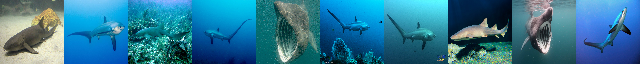
\includegraphics{lecture1_files/figure-beamer/cell-2-output-2.png}

}

\end{figure}
\end{frame}

\begin{frame}{Course Outline}
\protect\hypertarget{course-outline}{}
\begin{enumerate}
\tightlist
\item
  Mathematical and statistical modelling.
\item
  Brain modelling.
\item
  Simple neural networks and what they mean.
\item
  Developing primitive networks from scratch.
\item
  Developer tools: Flux; PyTorch; Tensorflow.
\item
  Developing complex deep learning models.
\end{enumerate}
\end{frame}

\begin{frame}{Data}
\protect\hypertarget{data}{}
\begin{itemize}
\item
  Data is typically anything we can measure.
\item
  It often is categorised by a set of real numbers (1.2, -1.4) and units
  (meters/second, red).
\item
  The quantisation of data is useful because it allows us to perform
  formal mathematical operations on it.
\end{itemize}
\end{frame}

\begin{frame}{Probability}
\protect\hypertarget{probability}{}
\begin{itemize}
\item
  Probability is a number we use to characterise the likelihood of an
  event.
\item
  The probability can be thought of as the proportion of times we expect
  this event to happen asymptotically. (Debate)
\item
  The probability of standard a die rolling 1 is 1/6.
\end{itemize}
\end{frame}

\begin{frame}{Distribution}
\protect\hypertarget{distribution}{}
\begin{itemize}
\item
  A distribution is the probabilitisc description of \emph{all} possible
  events.
\item
  Distributions may be discrete (categorical) or continuous.
\item
  All elements in the distribution must integrate to a total probability
  of 1.
\item
  A distribution is often parameterised by a series of numbers:
  \(\vec{\beta}\)
\end{itemize}
\end{frame}

\begin{frame}{PDFs and CDFs}
\protect\hypertarget{pdfs-and-cdfs}{}
\begin{itemize}
\item
  Distributions can be described with a probability density function
  (PDF) or cummulative density function (CDF):
  \[CDF(x) = \int_{\infty}^x PDF(y) dy.\]
\item
  We can sample from a distribution using the inverse of the CDF.
\item
  We tend to describe random variables in terms of their distributions:
  \[X \sim D(\vec{\beta}) \]
\end{itemize}
\end{frame}

\begin{frame}{Data as a Distribution}
\protect\hypertarget{data-as-a-distribution}{}
\begin{itemize}
\item
  We can think of data as being described by a distribution.
\item
  A distribution is therefore a data generating process.
\item
  Each data point (an image, a measurement of velocity) is a random
  sample from some (potentially unknown distribution)
\end{itemize}
\end{frame}

\begin{frame}{Empirical Distributions}
\protect\hypertarget{empirical-distributions}{}
\begin{itemize}
\item
  We can use data samples to inform us about distributions.
\item
  The most naive thing to say is that the data \emph{is} the
  distribution.
\item
  The distribution is then defined by N data points and the CDF
  increases by \(1/n\) for each data point.
\end{itemize}
\end{frame}

\begin{frame}{}
\protect\hypertarget{section}{}
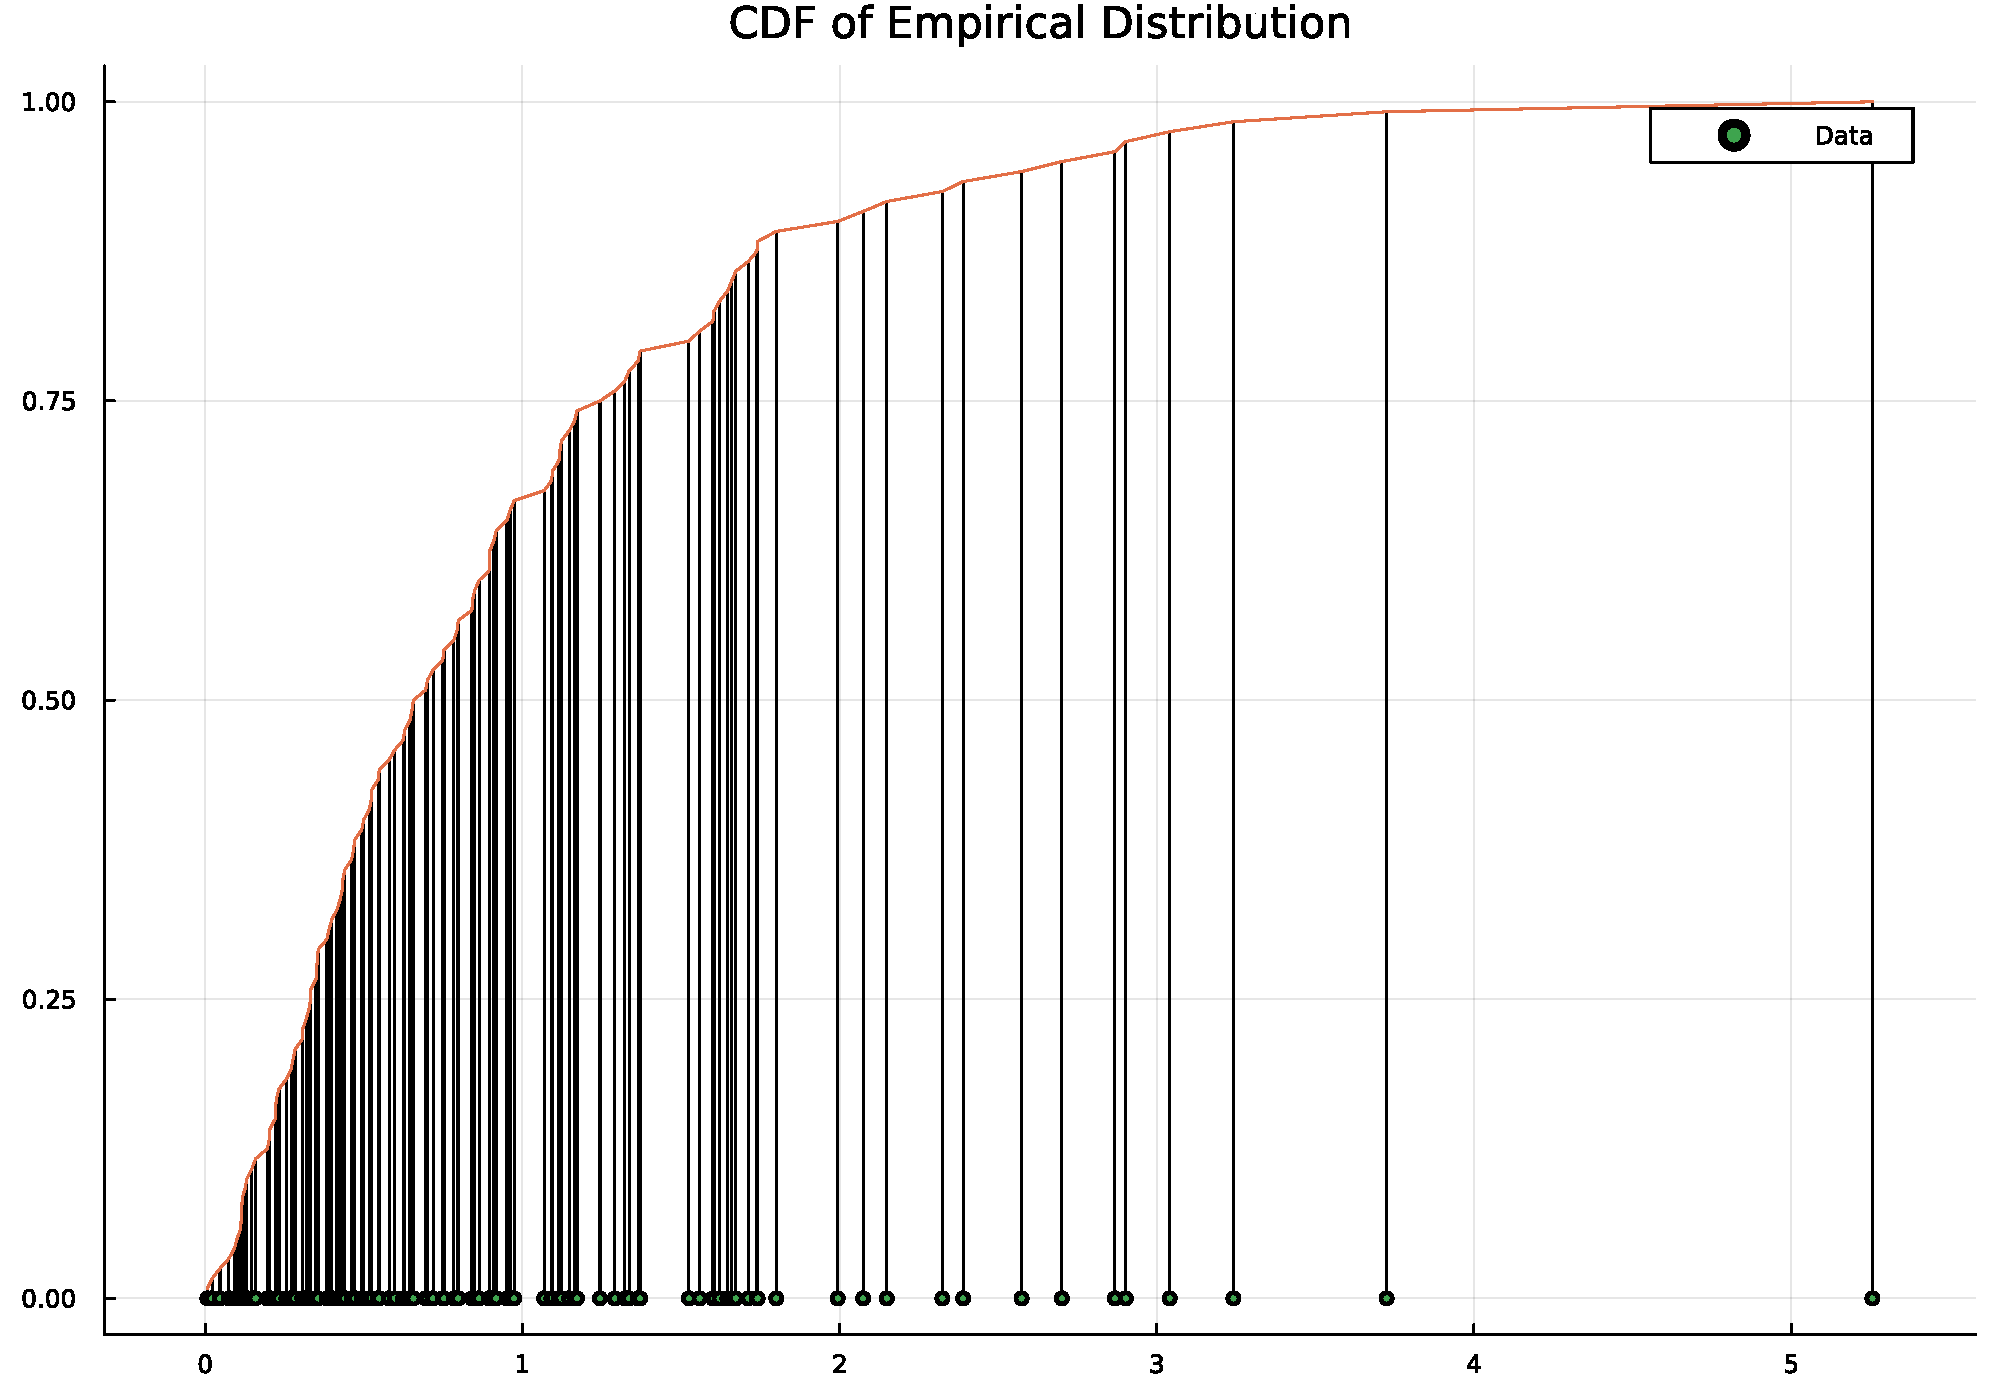
\includegraphics{lecture1_files/figure-beamer/cell-3-output-1.pdf}
\end{frame}

\begin{frame}{Kernel Density Estimation}
\protect\hypertarget{kernel-density-estimation}{}
\begin{itemize}
\item
  We might also say that each datum represents a kernel probability
  function.
\item
  The kernel encodes the likelihood of sampling at that point
  e.g.~\(N(x,1/n)\).
\item
  The distribution may then be estimated by summing the kernels and
  normalising by the number of data.
\end{itemize}
\end{frame}

\begin{frame}{}
\protect\hypertarget{section-1}{}
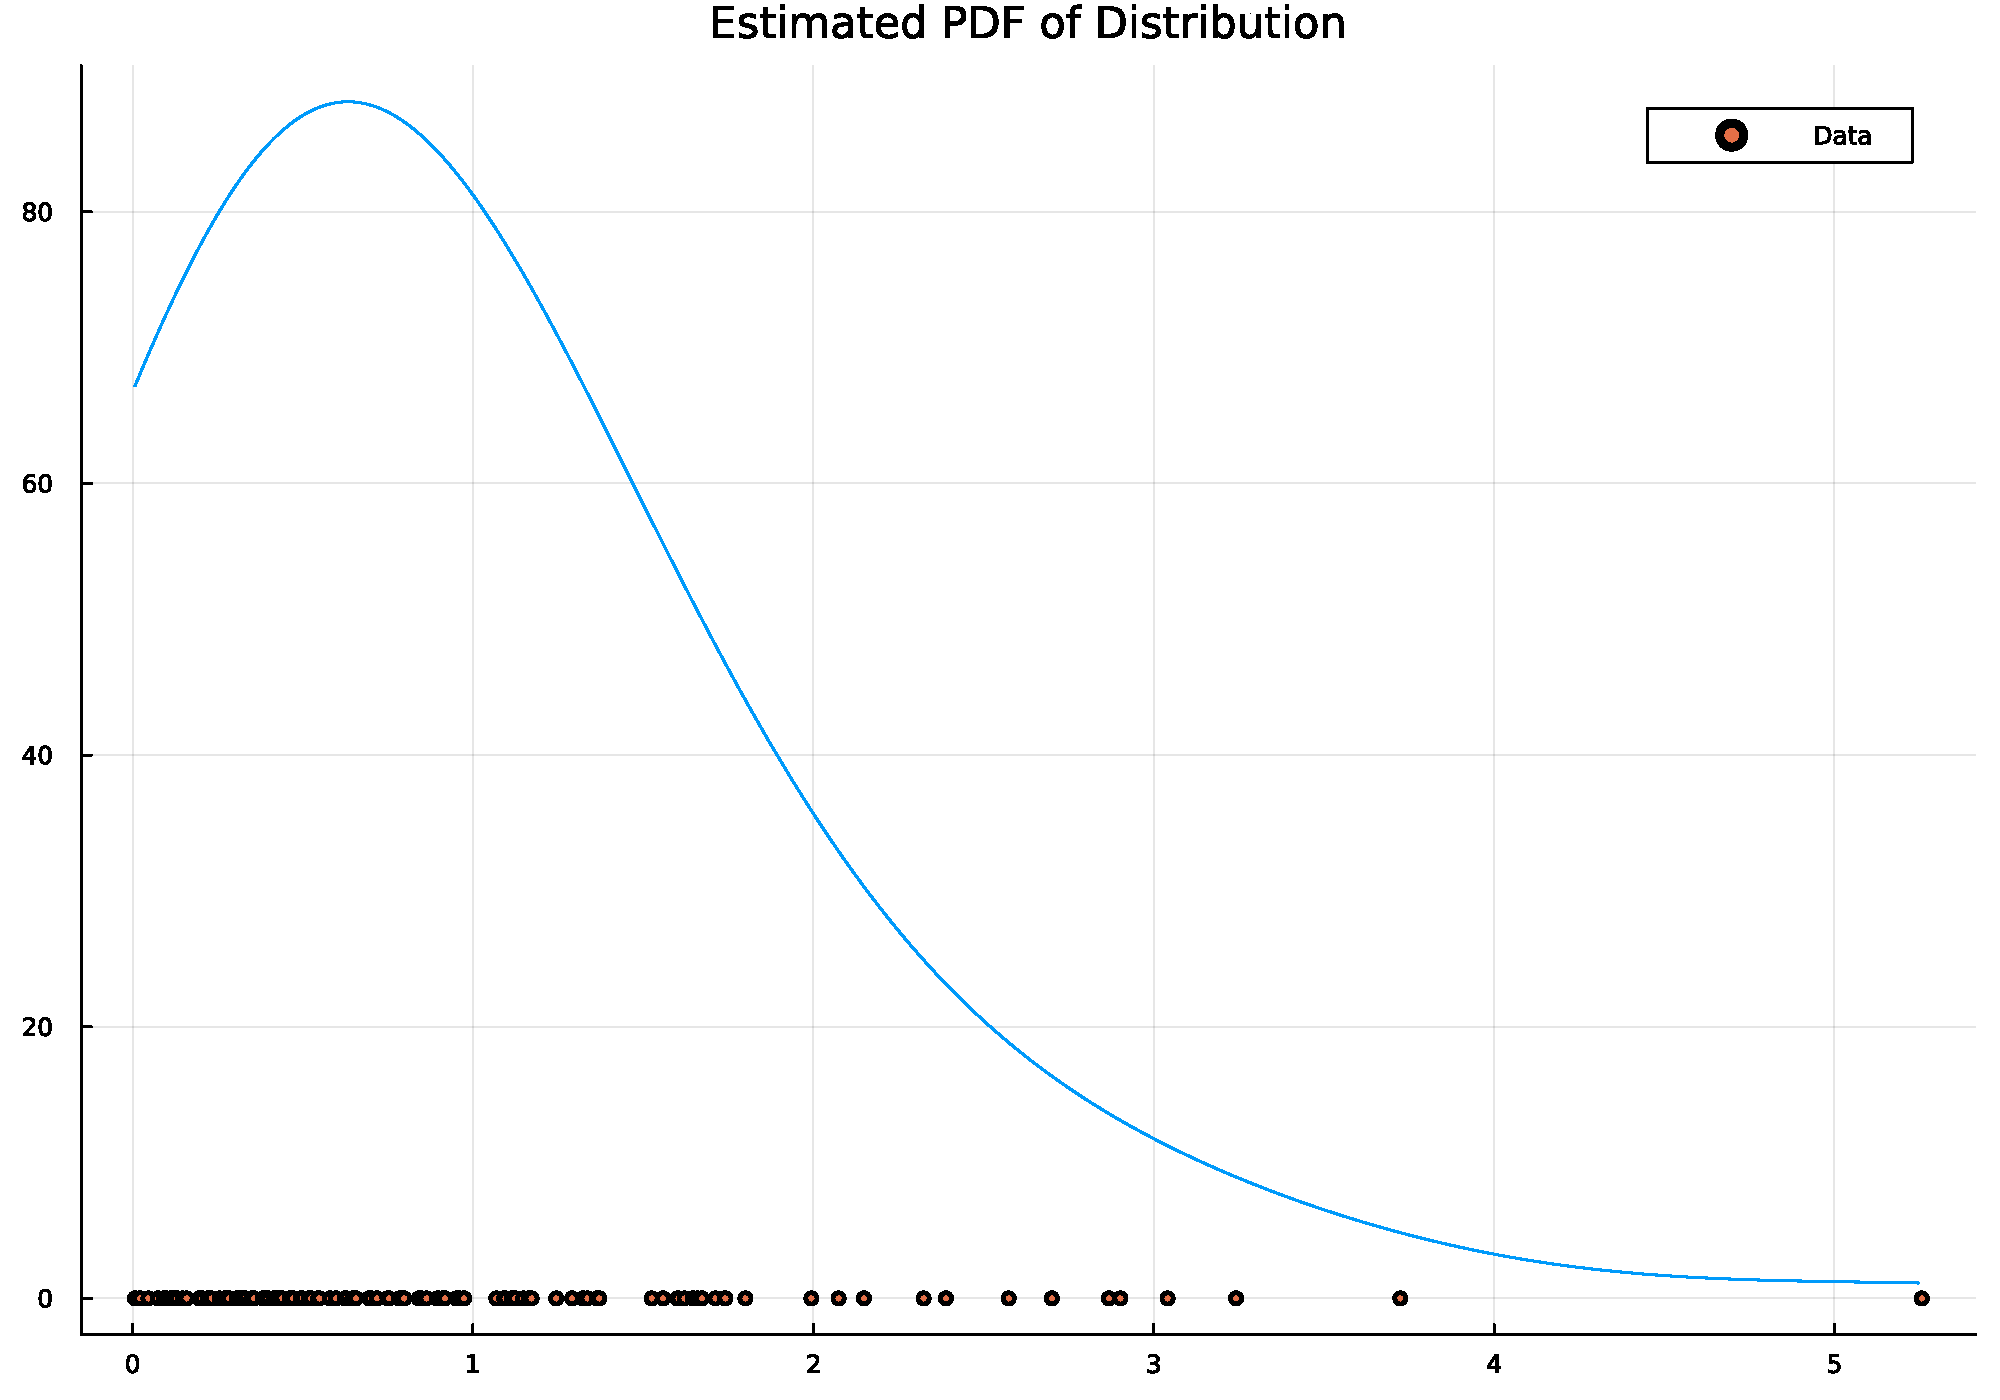
\includegraphics{lecture1_files/figure-beamer/cell-4-output-1.pdf}
\end{frame}

\begin{frame}{Statistics}
\protect\hypertarget{statistics}{}
\begin{itemize}
\item
  Data distributions can also be characterised by statistics.
\item
  Statistics are measurements that can be made on a data set.
\item
  They are also known (or can be estimated) for distributions.
\item
  The average, variance, standard deviation, quartiles, mode, and median
  are common examples.
\item
  A known distribution can be estimated using statistics: e.g
  \(N_{\text{est}}(\mu = \text{av}, \sigma^2 = \text{var})\)
\end{itemize}
\end{frame}

\begin{frame}{Central Limit Theorem}
\protect\hypertarget{central-limit-theorem}{}
\begin{itemize}
\item
  Central limit theorem: the mean of a collection of indepedent
  measurements tends towards a normal distribution.
\item
  Let \(\{X_i\}^n_{i=1}\) be iid from a distribution with mean \(\mu\)
  and variance \(\sigma^2\).
\item
  Suppose
  \(Z = \frac{\sum_i \frac{X_i}{n} - \mu}{\frac{\sigma}{\sqrt{n}}}\).
  Then, \(Z \sim N(0,1)\).
\item
  This is useful for analysing statistics (estimating distributions,
  regression, etc.)
\end{itemize}
\end{frame}

\begin{frame}{Modelling the Real World}
\protect\hypertarget{modelling-the-real-world}{}
\begin{itemize}
\item
  A model is a reduced description of real world phenenoma. They are
  \emph{always} wrong, but sometimes useful.
\item
  They are used to \emph{explain} and \emph{predict} aspects of that
  phenenoma.
\item
  They can be words, pictures, mental, mathematical, or
  algorithmic/computational.
\item
  We like mathematical and computational models because they are
  \emph{precise} i.e.~no ambiguity and falsifiable by experiment.
\end{itemize}
\end{frame}

\begin{frame}{Mathematical and Computational Models}
\protect\hypertarget{mathematical-and-computational-models}{}
\begin{itemize}
\item
  The general form of a precise model is a functional relationship.
\item
  The model (f) takes input (x) and as a black box produces output (y):
  \(y = f(x)\)
\item
  The science (or description) is encoded in the definition of x.
\end{itemize}
\end{frame}

\begin{frame}{Statistical Models}
\protect\hypertarget{statistical-models}{}
\begin{itemize}
\item
  We would like to relate our measured data to each other.
\item
  We do this by asserting that there is a model between the relevant
  data.
\item
  Then, we precisely formulate this model in the form of a mathematical
  function.
\item
  We typically manipulate an \emph{indepedent} variable (x) and measure
  the \emph{depedent} variable (y).
\item
  We \emph{assume} with some random error \(\epsilon\):
  \[y_i = f(x_i) + \epsilon\]
\end{itemize}
\end{frame}

\begin{frame}{Transformed Distribution}
\protect\hypertarget{transformed-distribution}{}
\begin{itemize}
\item
  We can also query the statistics of the transformed variable (y =
  f(x)) under the model: \[ F_Y(y(x)) = F_X(x)\]
\item
  Differentiating CDFs gives PDFs:
  \[ \frac{\partial}{\partial x} F_Y(y(x)) = f_X(x)\]
\item
  Using the chain rule yields:
  \[ f_Y(y) = \left|\frac{\partial y}{\partial x}\right|^{-1} f_X(x) \]
\end{itemize}
\end{frame}

\begin{frame}{Models are Data Generating}
\protect\hypertarget{models-are-data-generating}{}
\begin{itemize}
\item
  We can think of a model as a data generating process.
\item
  A measurement is made with some error: it is a sample from a
  distribution.
\item
  Data is a linearly indepedent collection of measurements. (Central
  Limit Theorem)
\item
  Model makes predictions by transforming the indepedent measurements.
  Depedent measurements come from the \emph{true} process.
\item
  Models \emph{often} (not necessarily) take some natural law form of
  this process e.g.~\(x(t) = x_0 + vt\)
\end{itemize}
\end{frame}

\begin{frame}{Parameters and Hyperparameters}
\protect\hypertarget{parameters-and-hyperparameters}{}
\begin{itemize}
\item
  A model is characterised by a series of numbers that are not data.
\item
  These are typically called \emph{parameters} e.g.~\(v, x_0\) in
  \(x(t) = x_0 + v t\).
\item
  A models parameters may come from a distribution and these are
  referred to as \emph{hyper-parameters}
\item
  Hyper-parmaters can also refer to parameterisations that are part of
  the model specification e.g.~fitting.
\end{itemize}
\end{frame}

\begin{frame}{Estimating Parameters}
\protect\hypertarget{estimating-parameters}{}
\begin{itemize}
\item
  We generally use data to try and estimate the parameters of a model.
\item
  This is a procedure known as \emph{fitting}.
\item
  Fitting typically involves minimising a quantity between predictions
  and measurements.
\end{itemize}
\end{frame}

\begin{frame}{Bayesian Statistics vs Frequentists}
\protect\hypertarget{bayesian-statistics-vs-frequentists}{}
\begin{itemize}
\item
  Frequentist statistics assume estimates are true in the limiting value
  of large data.
\item
  Bayesian statistics assume that an estimate has a probability and data
  updates the probability via Bayes rule:
  \[p(\alpha | \text{data}) =\frac{ p( \text{data} | \alpha) p(\alpha) }{\text{data}}\].
\item
  \(p(\alpha | \text{data})\) is the \emph{posterior} probability model
  after observration
\item
  \(p(\alpha)\) encodes the \emph{prior} belief that a parameter
  \(\alpha\) follows a given distribution.
\item
  Bayesian statistics allow us to encode uncertainty into our data and
  treat our data and parameters as distributions.
\end{itemize}
\end{frame}

\begin{frame}{Model Fits}
\protect\hypertarget{model-fits}{}
\begin{itemize}
\item
  A model relates the distribution of the indepedent/depedent variables.
\item
  We also sample these distributions in the form of data.
\item
  We generally want to minimise some quantity error quantity between
  these two.
\item
  For example this could be minimising least squared error, or
  likelihood maximisation under a given model.
\end{itemize}
\end{frame}

\begin{frame}{Goodness of fit}
\protect\hypertarget{goodness-of-fit}{}
\begin{itemize}
\item
  To assess the goodness of fit we usually look at the difference
  between these distributions.
\item
  Most often this is done through the covariance
  e.g.~\[ r^2_{\text{Pearsons}} = \frac{\text{Cov}(X,Y)}{\sigma_X \sigma_Y}\]
\item
  Be careful with goodness of fit. Pearsons for example will only be
  meaningful for linear regression.
\item
  Many other measures, some penalise number of parameters e.g.~Akaike
  Information Criterion.
\end{itemize}
\end{frame}

\begin{frame}{Linear Regression}
\protect\hypertarget{linear-regression}{}
\begin{itemize}
\item
  Linear regression is the most common form of model fitting.
\item
  It assumes that the \emph{parameters} are linear in the model.
\item
  The regressors (depedent variables) may still be non linear
  e.g.~\(y = \beta_0 + \beta_1 x + \beta_2 x^2\)
\end{itemize}
\end{frame}

\begin{frame}{Linear Regression Format}
\protect\hypertarget{linear-regression-format}{}
\begin{itemize}
\item
  The general form of a linear model is: \[ \vec{Y} = W \vec{X} \]
\item
  \(\vec{X}\) is an N dimensional vector of features (indepedent
  variables; \(x_i\), \(x_i^2\), \(x_ix_j\) etc.)
\item
  \(\vec{Y}\) is an M dimensional vector of responses (dependent
  variables)
\item
  \(W\) is a design matrix which relates the regressors (indepdent
  variables) to the observables (dependent variables).
\end{itemize}
\end{frame}

\begin{frame}{Weights and Biases}
\protect\hypertarget{weights-and-biases}{}
\begin{itemize}
\item
  The 0th component of the design matrix often incorporates the 0
  reponse variable.
\item
  This is the ``intercept'' of the model and when designed this way the
  feature vector is prepended with a 1 (a valid constant regressor).
\item
  This can also be taken out and referred to as the biases:
  \[ Y = W X + b\].
\item
  Weights and biases are a common way to refer to the parameters of the
  model.
\item
  Biases indicates how biased each response variable is.
\end{itemize}
\end{frame}

\begin{frame}{Linear Regression Error}
\protect\hypertarget{linear-regression-error}{}
\begin{itemize}
\item
  We need a procedure to perform the fit i.e.~we need an error function.
\item
  We choose the error between an observered regressor \(Y_j\) predicted
  regressor \(\hat{Y}_j = W X_n + B\) as the least squared error:
  \[ e_j = \text{sum}((\hat{Y_j}-Y_j).^2) \]
\item
  The total error which we want to minimise is: \[E = \sum_j e_j\]
  \[E = \sum_j \text{sum}(W X_j - Y_j).^2\]
\end{itemize}
\end{frame}

\begin{frame}{Minimise the error.}
\protect\hypertarget{minimise-the-error.}{}
\begin{itemize}
\item
  Consider the minimisation problem with just one data point.
\item
  This has a quadratic function form \(f(x,y) = (Wx-y)^2\).
\item
  We can reliably get to the ``bottom'' of a quadratic using basic
  calculus setting the gradient to zero.
\item
  The gradient here is easy to calculate: \(2(Wx - y)(Wx-y)^T\)
\end{itemize}
\end{frame}

\begin{frame}{Total error}
\protect\hypertarget{total-error}{}
\begin{itemize}
\item
  The total error is linear in each of the data points: we can just sum
  up the minmima simultaneously.
\item
  For a matrix of feature vectors \(\textbf{X}\) and responses
  \(\textbf{Y}\) we have: \[E =  (\textbf{X} W - \textbf{Y})^2\]
  \[\frac{dE}{dw} = 2(\textbf{X}w - \textbf{W})(\textbf{X}W - \textbf{Y})^T = 0\]
  \[ W = (\textbf{X}^T \textbf{X})^{-1} \textbf{X}^T \textbf{Y} \]
\item
  This is the optimal weights to minimise the mean squared error.
\end{itemize}
\end{frame}

\begin{frame}[fragile]{Example}
\protect\hypertarget{example}{}
\begin{Shaded}
\begin{Highlighting}[]
\NormalTok{x }\OperatorTok{=} \FunctionTok{hcat}\NormalTok{(}\FunctionTok{ones}\NormalTok{(}\FloatTok{50}\NormalTok{), }\FunctionTok{rand}\NormalTok{(}\FloatTok{50}\NormalTok{))}\CharTok{\textquotesingle{};}
\NormalTok{y }\OperatorTok{=}\NormalTok{ [}\FloatTok{1} \FloatTok{2}\NormalTok{] }\OperatorTok{*}\NormalTok{ x }\OperatorTok{.+} \FloatTok{0.04} \OperatorTok{*} \FunctionTok{rand}\NormalTok{(}\FloatTok{1}\NormalTok{, }\FunctionTok{size}\NormalTok{(x)[}\FloatTok{2}\NormalTok{]);}
\NormalTok{W }\OperatorTok{=}\NormalTok{ (}\FunctionTok{inv}\NormalTok{(x}\OperatorTok{*}\NormalTok{x}\OperatorTok{\textquotesingle{}}\NormalTok{) }\OperatorTok{*}\NormalTok{ (x}\OperatorTok{*}\NormalTok{y}\OperatorTok{\textquotesingle{}}\NormalTok{))}\CharTok{\textquotesingle{};}
\end{Highlighting}
\end{Shaded}

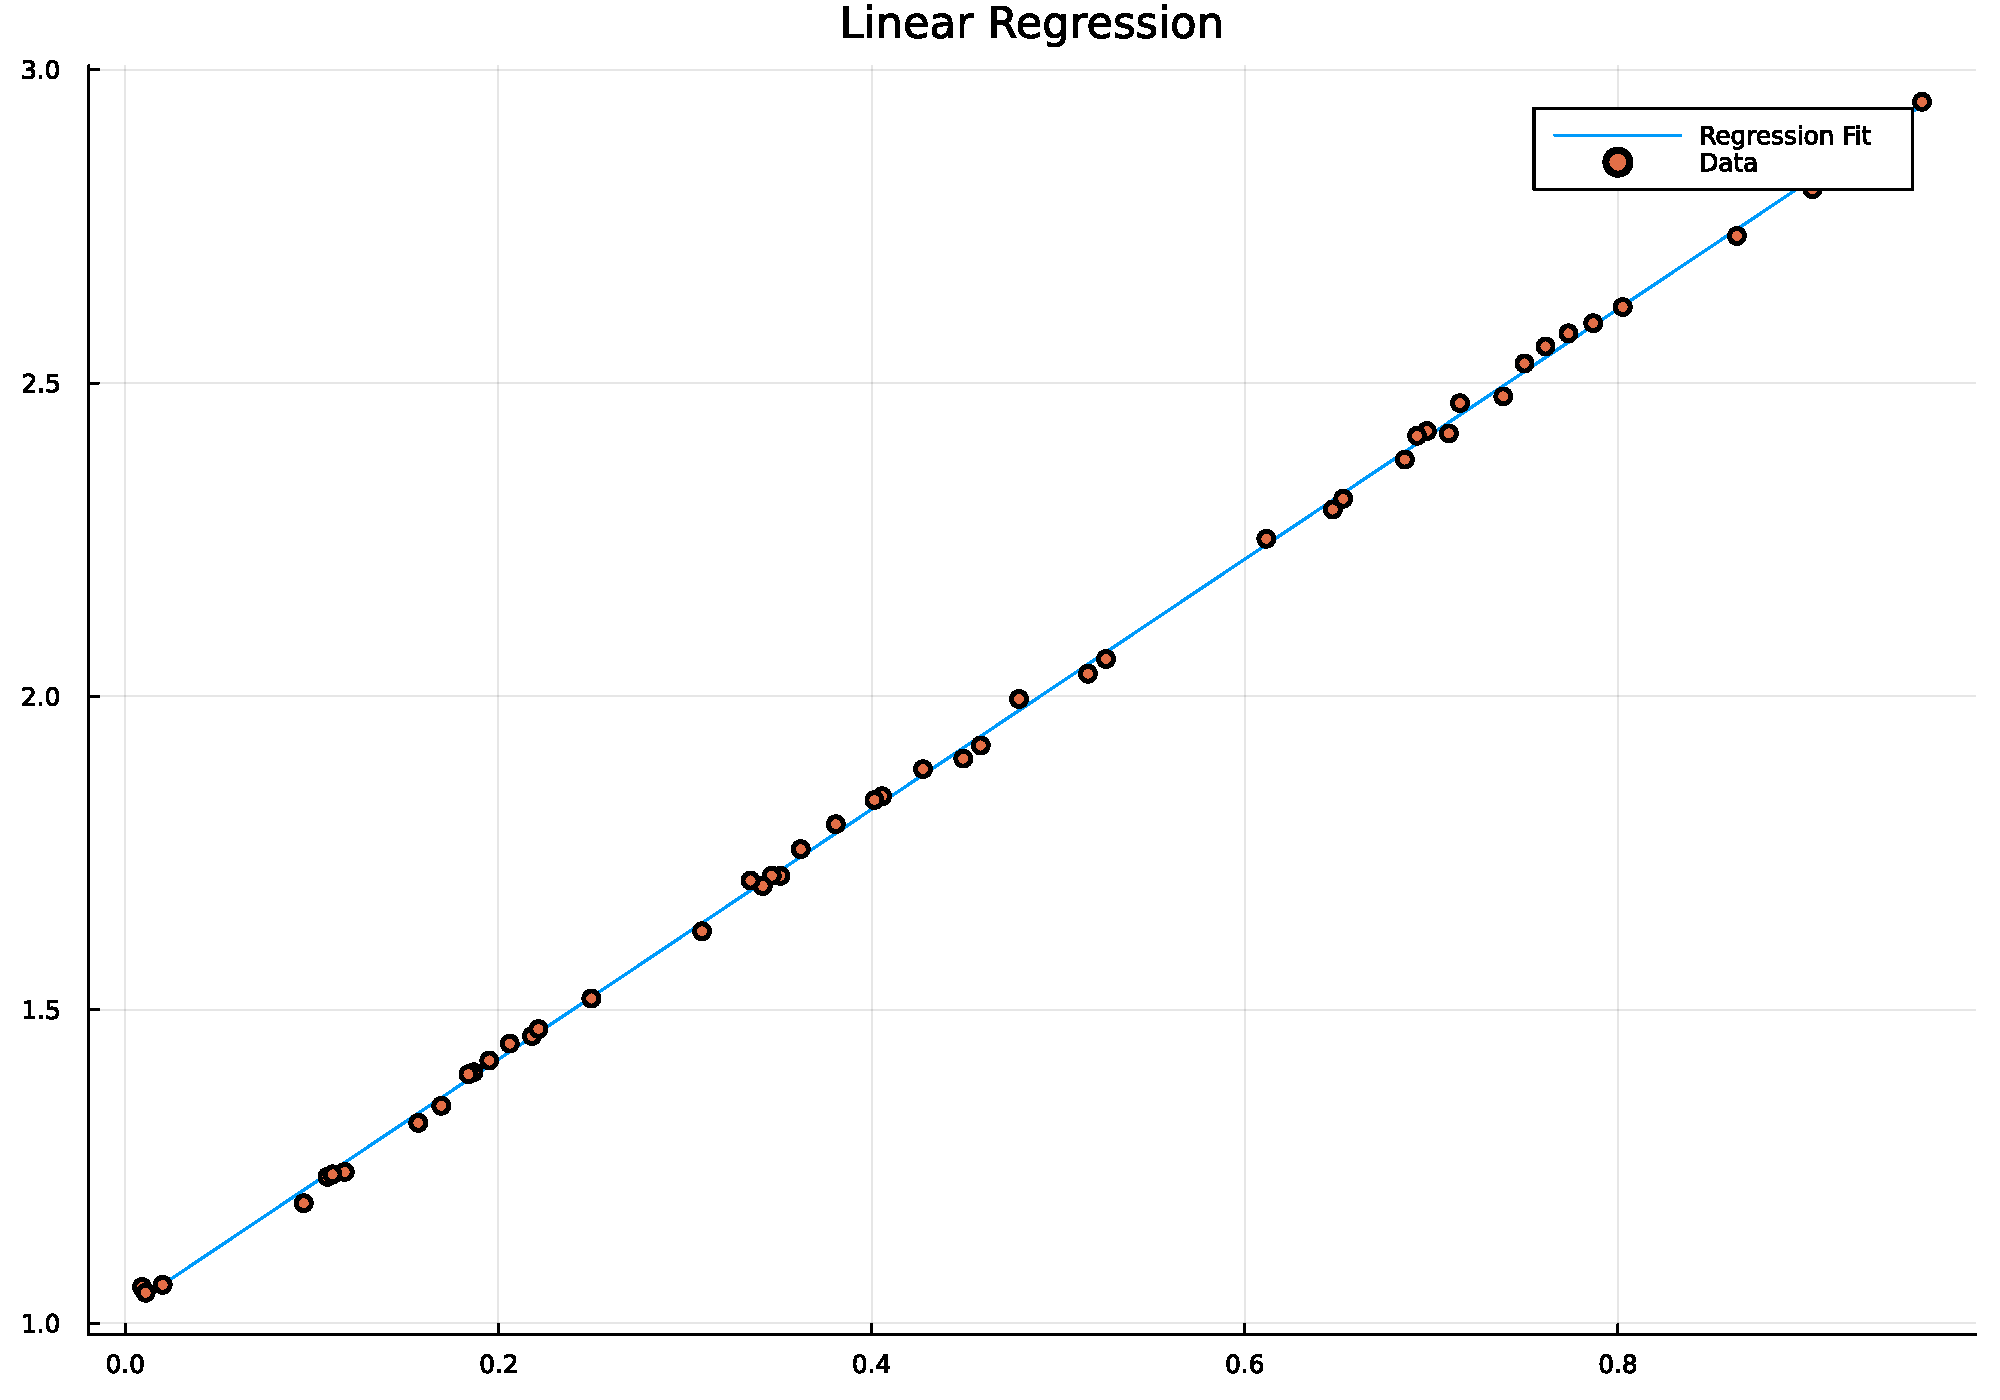
\includegraphics{lecture1_files/figure-beamer/cell-7-output-1.pdf}
\end{frame}

\begin{frame}{Nonlinear Regression}
\protect\hypertarget{nonlinear-regression}{}
\begin{itemize}
\item
  Nonlinear regression allows the model to be non-linear in the
  parameters
  e.g.~\[ f(x; \alpha, \beta) = \frac{x^n}{\alpha x^n + \beta^2} \].
\item
  Nonlinear regression is generally more difficult to interpret: careful
  with goodness of fits.
\item
  A common non-linear function we want to fit is the logistic function.
\end{itemize}
\end{frame}

\begin{frame}{Logistic Function}
\protect\hypertarget{logistic-function}{}
\begin{itemize}
\item
  The logistic function is the solution to logistic equation often
  parameterised as:
  \[ p(x; \mu, \sigma) = \frac{1}{1 + \exp\left(\frac{\mu-x}{\sigma}\right)} \]
\item
  It typically is interpreted to give a probability that is used to
  classify a variable.
\item
  It comes up often in nature e.g.~the firing response of a neuron.
\item
  The logit is the inverse of the logistic function.
\end{itemize}
\end{frame}

\begin{frame}{Logistic Regression}
\protect\hypertarget{logistic-regression}{}
\begin{itemize}
\item
  Logistic regression attempts to estimate the parameters of the
  logistic function.
\item
  Suppose \(y \in \{0,1\}\) and p(x) gives the probability of y. The
  cross entropy of the ith datapoint is defined as:
  \[-y_i \ln(p(x_i)) - (1-y_i) \ln(1-p(x_i))\]
\item
  It is zero if and only if all predictions are corrected. Otherwise it
  measures the entropy (think, disarray) between the two distributions.
\item
  The parameters that minimise the cross-entropy are the best fit and
  are solved numerically through \emph{gradient descent}; covered later.
\end{itemize}
\end{frame}

\begin{frame}{Regression, Classification, and Generation}
\protect\hypertarget{regression-classification-and-generation}{}
\begin{itemize}
\item
  Suppose that we have fitted our statistical model. The utility is in
  its \emph{prediction}.
\item
  The predictions are all technically regressions but are thought of in
  three categeries: regression, classification, and generation.
\item
  Regression is the model output given some known choice of independent
  variable.
\item
  Classification is the discrete model ouput (often the maximum
  probability) representing a category.
\item
  Generation is the model output for some random (unseen) variable in
  the input space.
\end{itemize}
\end{frame}

\begin{frame}{Data Preprocessing}
\protect\hypertarget{data-preprocessing}{}
\begin{itemize}
\item
  Often we find ourselves \emph{exploring} data before we generate
  models on it.
\item
  There are many useful techniques that can be applied to data.
\item
  Noise reduction is an example of \emph{data cleaning}.
\item
  Clustering is a form of \emph{unsupersived learning}.
\item
  Principal Component Analysis is a form of \emph{dimensionality
  reduction}.
\end{itemize}
\end{frame}

\begin{frame}[fragile]{Clustering}
\protect\hypertarget{clustering}{}
\begin{itemize}
\item
  Clustering involves partitioning a dataset into a series of different
  groups.
\item
  This is generally done without labels and involves simple operations
  on the raw data.
\item
  Clustering algorithms are themselves powerful statistical models but
  they wont be covered in this course.
\item
  Common algorithims: \texttt{k-means} and \texttt{t-sne}.
\end{itemize}
\end{frame}

\begin{frame}{Dimensionality Reduction}
\protect\hypertarget{dimensionality-reduction}{}
\begin{itemize}
\item
  Often data is very high-dimensional but these dimensions dont convey
  much information.
\item
  Dimensionality reduction is a change of variables that captures most
  of the information with just a few variables.
\item
  This can drastically simplify models.
\end{itemize}
\end{frame}

\begin{frame}{Principal Component Analysis}
\protect\hypertarget{principal-component-analysis}{}
\begin{itemize}
\item
  Principal Component Analysis is a very popular dimension reduction
  technique.
\item
  It works by transforming the variables into a maximal variance
  encoding.
\item
  This is achieved by eigenvalue decomposition of the covariance matrix.
\item
  The principal eigenvector contains the most variance, and so on.
\end{itemize}
\end{frame}

\begin{frame}{Learning}
\protect\hypertarget{learning}{}
\begin{itemize}
\item
  Learning in the context of statistics refers to correctly
  parameterising a model.
\item
  It is generally an iterative process where data is repeatedly
  presented to a learning algorithm.
\item
  It is usually described as unsupervised when the data has not been
  ``tagged'' and supervised when it has.
\item
  In supervised learning we know the ``right'' answer and can therefore
  construct a reasonable sense of error e.g.~least squares.
\item
  Clustering is unsupervised; linear regression is supervised.
\end{itemize}
\end{frame}

\begin{frame}{Deep Learning?}
\protect\hypertarget{deep-learning}{}
\begin{itemize}
\item
  This has been a lot of general statistics. What does it have to do
  with Deep Learning?
\item
  At the heart of all machine learning is distribution matching.
\item
  Deep learning is just a powerful class of general non-linear
  statistical models.
\item
  The model format takes inspiration from a physical structure (like
  most models) - the brain.
\item
  We will go over this physical inspiration in the following lecture.
\end{itemize}
\end{frame}

\begin{frame}{Summary}
\protect\hypertarget{summary}{}
\begin{itemize}
\item
  Data is the entry point of all sciences.
\item
  Models are precise and experimentally falsifiable relationships
  between data.
\item
  Models are used for prediction and explanation.
\item
  Deep Learning models are complex non-linear statistical models
  inspired by the brain.
\end{itemize}
\end{frame}



\end{document}
